\section{Details of the Experiment Setup}
\label{appendix:experiment_setup_detail}

\paragraph{Models in Baseline RAG Systems} 
We use the version of \texttt{e5-mistral-7b-instruct} for the E5-Mistral retriever. For the generators, we use \texttt{gpt-4-turbo-2024-04-09} version for GPT-4, \texttt{Llama3-8B-Instruct} for Llama3-8B and \texttt{Llama3-70B-Instruct} for Llama3-70B, and \texttt{Mixtral-8x7B-Instruct-v0.1} for Mixtral-8x7B. 

We adopt OpenSearch\footnote{\url{https://opensearch.org/}} as the tool to implement the inverted index for BM25 and the approximate KNN search for dense retrieval. We use a g5.48xlarge instance with 8 NVIDIA A10G GPUs on AWS for inference of open-source models. We split documents in the corpus to chunks of 300 tokens with an overlap ratio of 0.2 by default. We use the tokenizer of E5-Mistral for both retrievers to control the chunking. For each query, top-20 chunks ranked by retrievers are used as context for LLM generation. The default prompt for all generators is shown in Fig.~\ref{fig:smiple_generation_prompt}. We set the generation temperature to 0.0 (deterministic) and the maximum generation length to 2,048 tokens when calling proprietary LLMs.% \begin{tcolorbox}[colback=OliveGreen!5!white,colframe=teal!75!black]
% Please answer the given question based on the context.\par
% \textcolor{awesome}{<context>}\par
% \textcolor{teal}{<content>}\par
% {$chunk_1$}\par
% \textcolor{teal}{</content>}\par
% \textcolor{teal}{<content>}\par
% {$chunk_2$}\par
% \textcolor{teal}{</content>}\par
% ...\par
% \textcolor{teal}{<content>}\par
% {$chunk_k$}\par
% \textcolor{teal}{</content>}\par
% \textcolor{awesome}{</context>}\par
% Question: {question}\\\\
% Please answer the question and tag your answer with <answer></answer>.
% \end{tcolorbox}


\begin{figure}
    \centering
    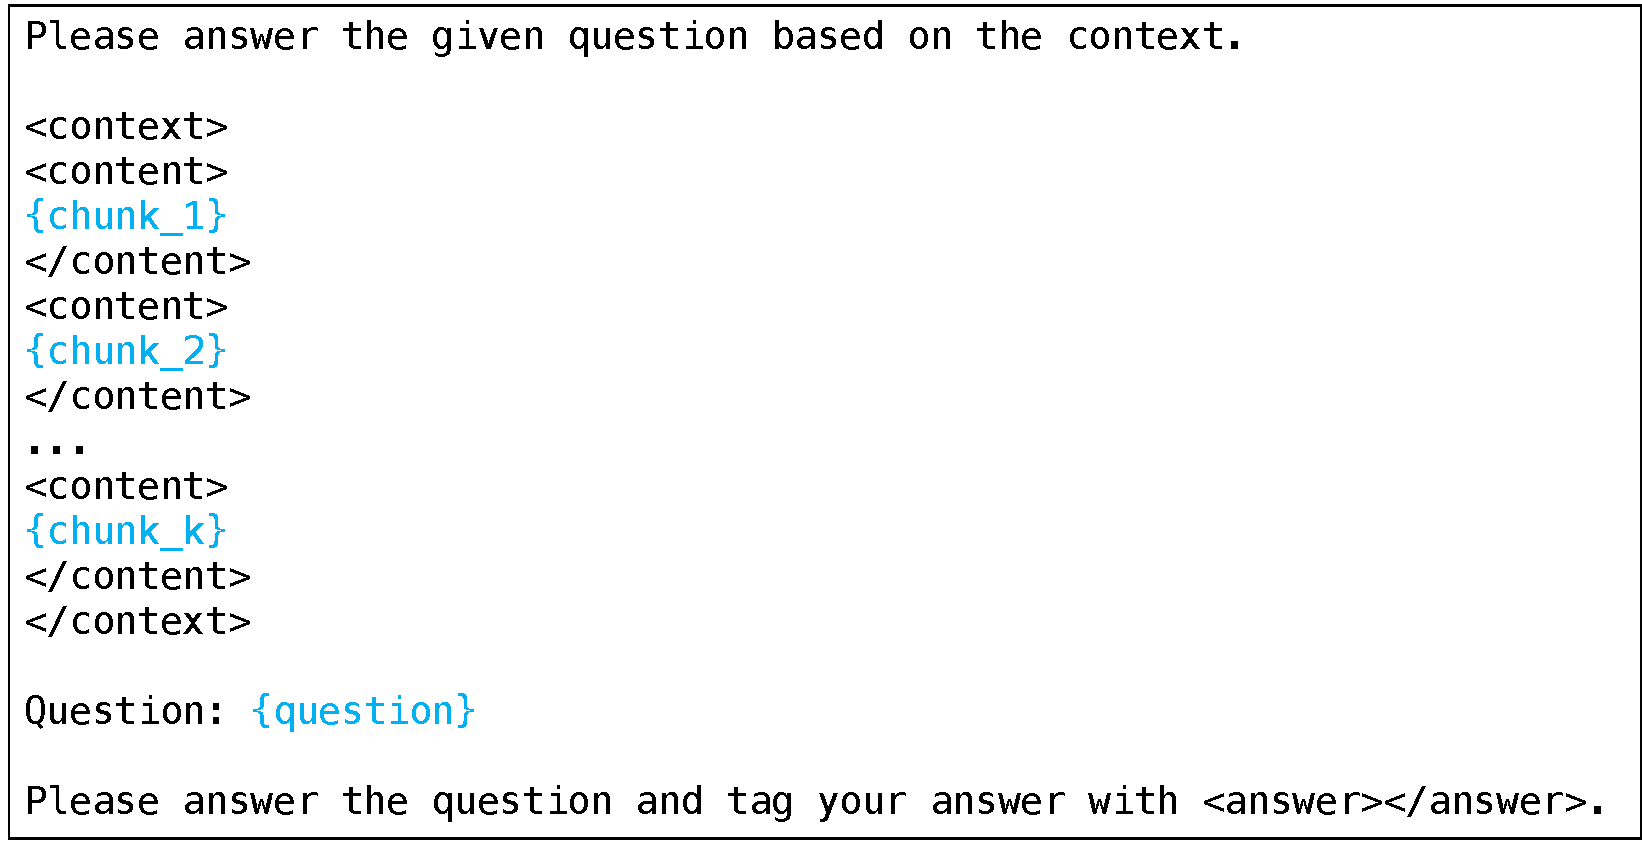
\includegraphics[width=0.8\textwidth]{figures/simple_generation_prompt.pdf}
    \caption{The default prompt used for response generation in the main experiments for the 8 RAG baseline systems.}
    \label{fig:smiple_generation_prompt}
\end{figure}



\section{Detailed Experiment Results}
\label{appendix:more_experiments}
The detailed evaluation results for all our benchmark datasets can be found in Tab.~\ref{tab:metrics_clapnq} to Tab.~\ref{tab:metrics_kiwi}.